\documentclass[11pt]{article}
\usepackage[margin=1in, top=0.3in]{geometry}
\usepackage[all]{nowidow}
\usepackage[hyperfigures=true, hidelinks, pdfhighlight=/N]{hyperref}
\usepackage[separate-uncertainty=true, group-digits=false]{siunitx}
\usepackage{graphicx,amsmath,physics,tabto,float,amssymb,pgfplots,verbatim,tcolorbox}
\usepackage{listings,xcolor,subfig,caption,import,wrapfig}
\usepackage[version=4]{mhchem}
\usepackage[noabbrev]{cleveref}
\newcommand{\creflastconjunction}{, and\nobreakspace}
\numberwithin{equation}{section}
\numberwithin{figure}{section}
\numberwithin{table}{section}
\definecolor{stringcolor}{HTML}{C792EA}
\definecolor{codeblue}{HTML}{2162DB}
\definecolor{commentcolor}{HTML}{4A6E46}
\captionsetup{font=small, belowskip=0pt}
\lstdefinestyle{appendix}{
    basicstyle=\ttfamily\footnotesize,commentstyle=\color{commentcolor},keywordstyle=\color{codeblue},
    stringstyle=\color{stringcolor},showstringspaces=false,numbers=left,upquote=true,captionpos=t,
    abovecaptionskip=12pt,belowcaptionskip=12pt,language=Python,breaklines=true,frame=single}
\lstdefinestyle{inline}{
    basicstyle=\ttfamily\footnotesize,commentstyle=\color{commentcolor},keywordstyle=\color{codeblue},
    stringstyle=\color{stringcolor},showstringspaces=false,numbers=left,upquote=true,frame=tb,
    captionpos=b,language=Python}
\renewcommand{\lstlistingname}{Appendix}
\pgfplotsset{compat=1.17}

\begin{document}

\begin{center}
    {\huge Digital methods for neutron pulse shape discrimination in EJ301 liquid scintillator detectors}\\
    \vspace{0.2in}
    \textbf{KDSMIL001 | 2021}

    \section*{Abstract}\label{sec:Abstract} % rough rn
    We investigate two digital methods of pulse shape discrimination for neutron and photon events in an EJ301 scintillator detector. Neutron events in these detectors tend to have a longer decay tail to the resulting signal than do photon events. Both methods take advantage of this fact. 
    
\end{center}

\section{Introduction}\label{sec:Introduction}
\par Many areas of research rely on the detection of particles, the details of which form the data that is analysed and investigated in order to corroborate or disprove theory. It is very important, when detecting a particle, that you are certain that the particle is what you think it is. When it comes to detecting neutrons, this is not as simple as it sounds. 
\par Liquid scintillator detectors are often used in neutron detection due to their flexibility when it comes to the shape and size of the material as well as their fast timing performance, but these detectors are also sensitive to gamma rays. Scintillator detectors work by emitting light at an energy roughly proportional to the energy of the incident ionising particle, but the constant of proportionality changes depending on the type of particle \cite{Knoll}. This light is then detected by the photoelectric effect and the resulting voltage pulse collected by instrumentation. Different types of particles also result in slightly different voltage pulse shapes. It is this difference that is exploited by pulse shape discrimination techniques. 
\par These techniques were developed at a time where computational power was lacking, as well as expensive, so they were implemented in analogue systems. These systems integrated the voltage over a long and short time window, then took the ratio of the two values. Neutrons interactions result in larger component of the long integral than photon interactions, so this ratio is different for these two types of interaction. Due to the nature of the electronics needed to integrate these pulses, the analysis had to be performed at run-time, which means the methods available were severely limited. Since computational power is now much more available and affordable, it no longer makes sense to use these analogue systems when the pulses could be captured digitally and analysed later, with much more freedom to experiment with different techniques, using the same data, in order to compare them. There are also more advanced techniques, such as decomposition of the decay curve into its individual exponential components, that are now possible.
\par This report will investigate the digital implementation of a technique similar to the one used in analogue systems, the Charge Comparison Method, as well as a new method that is only possible due to the digitisation of the data: the Pad\'e-Laplace Method. The data from two separate neutron sources, detected with a NE-213 liquid scintillator detector, will be analysed with these two methods in order to compare them based on the Figure of Merit described in Knoll (2010, p.701). The Charge Comparison Method is well understood and simple to implement but does not perform well at lower energies, so other methods must be investigated.

\section{Theory}\label{sec:Theory}
\subsection{Detecting Neutrons}
\par A distinction must be made between ``fast'' and ``slow'' neutrons as they interact with matter in distinct ways. The neutrons of interest in this paper are fast neutrons, with energies $\gtrsim1$ eV. These interact with matter by collisions, scattering off nuclei and depositing some fraction of their kinetic energy, or by inducing reactions in the target material. Slow neutrons, which are not accounted for in this paper, seem to have a much larger cross section of interaction than fast neutrons, which leads to some interesting applications and physics. The detection mechanisms developed for slow neutrons are thus very different to those used for fast neutrons. \cite{Knoll}
\begin{wrapfigure}{r}{0pt}
    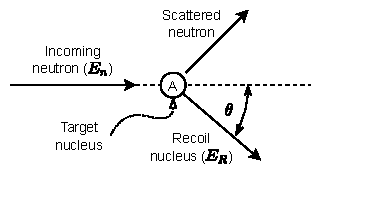
\includegraphics{Plots/neutronScattering.pdf}
    \caption{Elastic neutron scattering.}
    \label{fig:neutron scattering diagram}
\end{wrapfigure}
\par Fast neutrons can be detected in a few different ways, as discussed in Knoll (2010, ch.14-15), but when the energy of the neutrons is relevant there is only one mechanism of interest: elastic scattering. Neutrons collide with nuclei in the target material and transfer a fraction of their kinetic energy to the nucleus. The fraction of energy deposited is given by
\begin{equation}
    \frac{E_R}{E_n}=\frac{4A}{(1+A)^2}(\cos^2\theta)
    \label{eqn:Neutron scattering fraction}
\end{equation}
where $E_R$ is the energy deposited, $E_n$ is the energy of the incident neutron, $A$ is the mass of the target nucleus in neutron masses, and $\theta$ is the scattering angle of the recoil nucleus, relative to the incoming nucleus.
\par Scintillator detectors work by emitting light as a result of radiation exciting the detector material, whether that's single atoms or creating vibrations in the lattice of the material. Organic scintillator detectors, such as the NE-213 detector used in these experiments, work by the excitation of single atoms or molecules in the detector material. When it comes to neutrons, as seen by \cref{eqn:Neutron scattering fraction}, the mass of the target nuclei affects the fraction of energy that can be absorbed by the detector material. Hydrogen, which has a mass effectively equal to that of a neutron, is thus a very good candidate for absorption of a neutron's kinetic energy by elastic scattering. As a result of this, organic scintillator detectors with a large proportion of lone hydrogen atoms work well for detecting neutrons, especially when it comes to accurately detecting neutron energy.
\par 







%\par This section will include details from Knoll about liquid scintillator detectors, including the fact that different types of particles will result in different amounts of delayed fluorescence relative to prompt fluorescence. Neutrons seem to result in more than photons. Neutrons are detected by proton recoil events, while photons are detected by electron recoil events (Compton scattering), and hardly any photoelectric effect, so we only see Compton continuum, not photopeak.
\par 

\section{Methodology}\label{sec:Methodology}




\begin{thebibliography}{9}
    \bibitem{Knoll}

    \bibitem{Lang}
    
\end{thebibliography}

\end{document}